\documentclass[a4paper]{article}
\usepackage{amsmath,amssymb}
\usepackage{tcolorbox}
\usepackage{geometry}
\geometry{left=1cm,right=1cm,top=1cm,bottom=1.5cm}
\usepackage{multicol}
\usepackage{array}
\usepackage{tikz}
\usepackage[vlined,ruled,linesnumbered]{algorithm2e}
\usepackage{float}
\begin{document}
\title{Algorithm \& Complexity}
\date{}
\begin{multicols}{2}
\maketitle
\begin{tcolorbox}[title=Complexity Classes]
    \begin{equation*}
		\begin{aligned}
			1\prec \log\log n\prec \log n\prec \sqrt{n}\prec 2^{\log n}\prec n\prec \log (n!)\\= n\log n
			\prec n^2 \prec 2^n \prec 4^{n}\prec n!\prec (2n)!\prec 2^{n^2}\prec 2^{2^n}
		\end{aligned}
	\end{equation*}
\end{tcolorbox}

\tcbox[left=0mm,right=0mm,top=0mm,bottom=0mm,boxsep=0mm,lefttitle=3mm,
toptitle=1mm,bottomtitle=1mm,title=Sort Algorithms]{
    \begin{tabular}{c|m{4em}m{4em}m{4em}|m{3em}}
        \bfseries Algorithm &\bfseries Best Case &\bfseries Average Case &\bfseries Worst Case &\bfseries Space \\
        \hline
        Linear Search &  $\Omega(1)$  &  $O(n)$  &  $O(n)$  & $O(1)$  \\
        Binary Search &  $\Omega(1)$   &  $O(\log n)$ &  $O(\log n)$    &  $O(1)$ \\
        % Binary Search Avg Case:
        % \frac{1}{n}\sum_{i=1}^k i\times 2^{k-1}
        \hline
        Selection Sort &  $\Theta(n^2)$  &  $\Theta(n^2)$     &    $\Theta(n^2)$   &  $O(1)$ \\
        Bubble Sort   & $\Theta(n^2)$  &  $\Theta(n^2)$  &    $\Theta(n^2)$   &  $O(1)$ \\
        Insertion Sort &  $\Omega(n)$  &  $O(n^2)$  & $O(n^2)$ &  $O(1)$ \\
        % Insertion Sort Avg Case:
        % Half of the moving distance of the worst case.
        % \frac{n^2}{4} comp. \frac{n^2}{4} exch.
        \hline
        Merge Sort     &  $\Theta(n\log n)$  &  $\Theta(n\log n)$   &   $\Theta(n\log n)$    &  $O(n)$  \\
        % Merge Sort Recurrence: C(2^n) = 2C(2^{n-1}) + 2^n
        Quick Sort     &  $O(n\log n)$   &   $O(n\log n)$    &  $O(n^2)$   & $O(\log n)$  \\
        % Quick Sort Recurrence: nC_n = n(n+1) + 2(C_0+\cdots+C_{n-1}) => 1.39n\log n [Lab01/1]
        % Construct a permutation tree to prove that
        % there is no such algorithm to reduce 
        % the time complexity below O(\log(n!)) = O(n\log n)
    \end{tabular}
}

\begin{tcolorbox}[title=Master Theroem]
    \begin{equation*}
        T(n) = aT\left(\left\lceil\frac{n}{b}\right\rceil\right) + O(n^d)
    \end{equation*}
    \begin{equation*}
        T(n) = \begin{cases}
            O(n^d),&\text{if } d>\log_b a, \\
            O(n^d\log n), &\text{if } d=\log_b a,\\
            O(n^{\log_b a}), &\text{if } d<\log_b a.
        \end{cases}
    \end{equation*}
    \tcblower
    \begin{equation*}
        T(n) = aT\left(\frac{n}{b}\right) + f(n)
    \end{equation*}
    \begin{equation*}
        T(n) = \begin{cases}
            \Theta(n^{\log_b a}), &\exists \epsilon>0: f(n) = O(n^{\log_b a}-\epsilon)\\
            \Theta(n^{\log_b a}\lg n),&f(n)=\Theta(n^{\log_b a})\\
            \Theta(f(n)),&\exists \epsilon>0:f(n)=\Omega(n^{\log_b a+\epsilon}) \land \\&\exists c<1:af\left(\frac{n}{b}\right)\leq cf(n)
        \end{cases}
    \end{equation*}
\end{tcolorbox}

\begin{tcolorbox}[title=Sorting Network]
    \begin{tabular}{cc}
        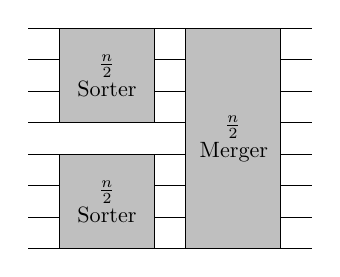
\begin{tikzpicture}[scale=0.8,every node/.style={scale=0.8}]
        \foreach \x in {1,...,8}
            \draw (1,0.5*\x) edge (5.5,0.5*\x);
        \draw[fill=gray!50]  (1.5,4) rectangle (3,2.5);
        \draw[fill=gray!50]  (1.5,2) rectangle (3,0.5);
        \draw[fill=gray!50]  (3.5,4) rectangle (5,0.5);
        \node[text width=3em,text centered] at (2.25,3.25) {$\frac{n}{2}$ Sorter};
        \node[text width=3em,text centered] at (2.25,1.25) {$\frac{n}{2}$ Sorter};
        \node[text width=3em,text centered] at (4.25,2.25) {$\frac{n}{2}$ Merger};
        \end{tikzpicture} & 
        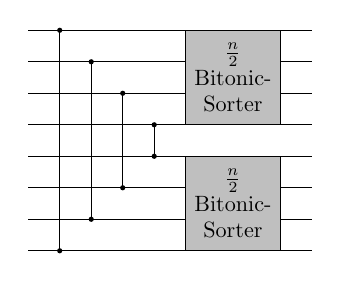
\begin{tikzpicture}[scale=0.8,every node/.style={scale=0.8}]
            \tikzstyle{bdot} = [fill=black,circle,scale=0.25];
            \foreach \x in {1,...,8}
                \draw (1,0.5*\x) edge (5.5,0.5*\x);
            \draw[fill=gray!50]  (3.5,4) rectangle (5,2.5);
            \draw[fill=gray!50]  (3.5,2) rectangle (5,0.5);
            \node[text width=4em,text centered] at (4.25,3.25) {$\frac{n}{2}$ Bitonic-Sorter};
            \node[text width=4em,text centered] at (4.25,1.25) {$\frac{n}{2}$ Bitonic-Sorter};
            \draw (1.5,4) node [bdot] {} -- (1.5,0.5) node [bdot] {};
            \draw (2,3.5) node [bdot] {} -- (2,1) node [bdot] {};
            \draw (2.5,3) node [bdot] {} -- (2.5,1.5) node [bdot] {};
            \draw (3,2.5) node [bdot] {} -- (3,2) node [bdot] {};
            \end{tikzpicture} \\
            Sorter($n$) & Merger($n$) \\
            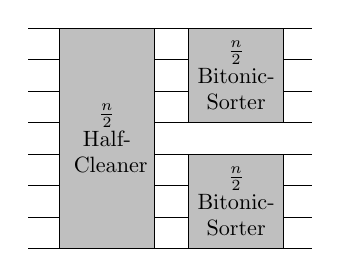
\begin{tikzpicture}[scale=0.8,every node/.style={scale=0.8}]
                \foreach \x in {1,...,8}
                    \draw (3,0.5*\x) edge (7.5,0.5*\x);
                \draw[fill=gray!50]  (5.55,4) rectangle (7.05,2.5);
                \draw[fill=gray!50]  (5.55,2) rectangle (7.05,0.5);
                \draw[fill=gray!50]  (3.5,4) rectangle (5,0.5);
                \node[text width=4em,text centered] at (6.3,3.25) {$\frac{n}{2}$ Bitonic-Sorter};
                \node[text width=4em,text centered] at (6.3,1.25) {$\frac{n}{2}$ Bitonic-Sorter};
                \node[text width=3em,text centered] at (4.25,2.25) {$\frac{n}{2}$ Half-Cleaner};
            \end{tikzpicture} &
            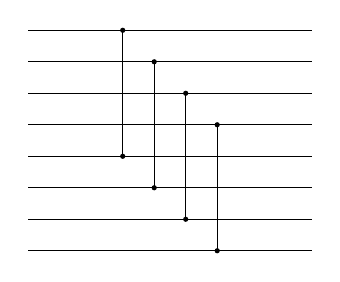
\begin{tikzpicture}[scale=0.8,every node/.style={scale=0.8}]
                \tikzstyle{bdot} = [fill=black,circle,scale=0.25];
                \foreach \x in {1,...,8}
                    \draw (1,0.5*\x) edge (5.5,0.5*\x);
                \draw (2.5,4) node [bdot] {} -- (2.5,2) node [bdot] {};
                \draw (3,3.5) node [bdot] {} -- (3,1.5) node [bdot] {};
                \draw (3.5,3) node [bdot] {} -- (3.5,1) node [bdot] {};
                \draw (4,2.5) node [bdot] {} -- (4,0.5) node [bdot] {};
            \end{tikzpicture} \\
            Bitonic-Sorter($n$) & Half-Cleaner($n$) \\
    \end{tabular}
    
\end{tcolorbox}

\begin{tcolorbox}[title=Greedy Algorithm]
    \begin{algorithm}[H]
        \caption{Interval Scheduling}
        Sort jobs by finish times so that $f_1\leq f_2\leq \cdots \leq f_n$\;
        $A\leftarrow \varnothing$\;
        \For{$j=1$ to $n$}{
            \If(){job $j$ is compatible with $A$}{
                $A\leftarrow A\cup \{j\}$\;
            }
        }
        \Return{$A$}\;
    \end{algorithm}
    \begin{algorithm}[H]
        \caption{Interval Partitioning}
        Sort intervals by starting time so that $s_1\leq s_2\leq \cdots \leq s_n$\;
        $d\leftarrow 0$\;
        \For{$j=1$ to $n$}{
            \If(){lecture $j$ is compatible with some classroom $k$}{
                schedule lecture $j$ in classroom $k$\;
            }
            \Else(){
                allocate a new classroom $d+1$\;
                schedule lecture $j$ in classroom $d+1$\;
                $d\leftarrow d+1$\;
            }
        }
        \Return{$A$}\;
    \end{algorithm}
    \begin{algorithm}[H]
        \caption{Minimize Lateness}
        Sort $n$ jobs by deadline so that $d_1\leq d_2\leq \cdots \leq d_n$\;
        $t\leftarrow 0$\;
        \For{$j=1$ to $n$}{
            Assign job $j$ to interval $[t,t+t_j]$\;
            $s_j\leftarrow t,f_j\leftarrow t+t_j$\;
            $t\leftarrow t+t_j$\;
        }
        \Return{interval $[s_j,f_j]$}\;
    \end{algorithm}
\end{tcolorbox}

% \begin{tcolorbox}[title=Greedy Analysis Strategies]
%     Greedy algorithm stays ahead.\\
%     Structural.\\
%     Exchange argument.
% \end{tcolorbox}

\begin{tcolorbox}[title=Matroid]
\paragraph{Independent System $(S,\mathbf{C})$} $$A\subset B, B\in \mathbf{C}\Rightarrow A\in \mathbf{C}$$
\paragraph{Matriod $(S,\mathbf{C})$}$$\begin{cases}
    (S,\mathbf{C})\text{ is an independent system,}\\
    A,B\in \mathbf{C} \land |A|<|B|\Rightarrow \exists x\in B\backslash A: A\cup \{x\}\in \mathbf{C}
\end{cases}$$ 
\paragraph{Maximal Independent subset $I$} $\not\exists x\not\in I: I\cup \{x\}$ is independent.
\begin{align*}
    u(F) &=\min\{|I||I\text{ is a maximal independent subset of }F\}\\
    v(F) &=\max\{|I||I\text{ is an independent subset of }F\}
\end{align*}
\paragraph{Matroid Theorem} an independent system $(S,\mathbf{C})$ is a matroid $\Leftrightarrow \forall F\subseteq S, u(F)=v(F)$.
\paragraph{Corollary} All maximal independent subsets in a matriod have the same size. 
\paragraph{Weighted Independent System $(S,\mathbf{C})$} with a nonnegative function $c:S\rightarrow \mathbb{R}^+$.
\end{tcolorbox}

\begin{tcolorbox}[title=Greedy-MAX]
    An independent system $(S,\mathbf{C})$ with cost function $c$, solving a maximization problem as:
    \begin{align*}
        \max~ &c(I)\\
        \text{subject to }& I\in\mathbf{C}
    \end{align*}
\begin{algorithm}[H]
    \caption{Greedy-MAX}
    Sort all elements in $S$ into ordering $c(x_1)\geq c(x_2)\geq \cdots \geq c(x_n)$\;
    $A\leftarrow \varnothing$\;
    \For{$i=1$ to $n$}{
        \If(){$A\cup \{x_i\}\in \mathbf{C}$}{
            $A\leftarrow A\cup \{x\}$\;
        }
    }
    \Return{$A$}\;
\end{algorithm}
% \paragraph{Theorem}
\begin{equation*}
    1\leq \frac{c(A^*)}{c(A_G)}\leq \max_{F\subseteq S}\frac{v(F)}{u(F)}
\end{equation*}
\paragraph{Corollary} If $(S,\mathbf{C},c)$ is a weighted matroid, then Greedy-MAX algorithm performs the optimal solution.
\end{tcolorbox}

\begin{tcolorbox}[title=Strongly Connected Components]
    \begin{algorithm}[H]
        Run DFS on $G^R$, and get the reversed visiting \texttt{order}\;
        % $n\leftarrow 0$\;
        % \ForEach(){$v$ in \texttt{order}}{
            Run DFS on $G$ within the visiting \texttt{order}\;
        %     $n\leftarrow n+1$\;
        % }
        % \Return{$n$}\;
        \caption{Kosaraju Algorithm}
    \end{algorithm}
\end{tcolorbox}

\begin{tcolorbox}[title=Dynamic Programming]
    \textbf{Optimal Substructure}\\\textbf{Overlapping subproblems}
    \begin{equation*}
        OPT(i,w) = \begin{cases}
            0, & j = 0,\\
            OPT(i-1,w), & w_i>w\\
            \max\{OPT(i-1,w),\\v_i+OPT(i-1,w-w_i)\}, &\text{else}.
        \end{cases}
    \end{equation*}
    \begin{algorithm}[H]
        \caption{Knapsack Algorithm 
        % using $n$-by-$W$ Array
        }
        \KwIn{$n,W,w_1,\cdots,w_n,v_1,\cdots,v_n$}
        \KwOut{Optimal value of knapsack with $W$}
        \For{$w\leftarrow 0$ to $W$}{
            $M[0,w]\leftarrow 0$\;
        }
        \For{$i\leftarrow 1$ to $n$}{
            \For(){$w\leftarrow 1$ to $W$}{
                \If(){$w_i>w$}{
                    $M[i,w]\leftarrow M[i-1,w]$\;
                }
                \Else(){
                    $M[i,w]\leftarrow \max\{M[i-1,w],v_i+M[i-1,w-w_i]\}$\;
                }
            }
        }
        \Return{$M[n,W]$}\;
    \end{algorithm}
    Running time is $\Theta(nW)$: ``pseudo-polynomial''.
\end{tcolorbox}

\begin{tcolorbox}[title=Linear Programming]
    \begin{multicols}{2}
        \paragraph{Primal Form}
        \begin{align*}
            \max& \sum_{j=1}^n c_jx_j \\
            s.t. & \sum_{j=1}^n a_{ij}x_j\leq b_i, &\forall i\\
                & x_j\geq 0,& \forall j
        \end{align*}
        \paragraph{Dual Form}
        \begin{align*}
            \max& \sum_{i=1}^n b_iy_i \\
            s.t. & \sum_{i=1}^m a_{ij}y_i\leq v_j, &\forall j\\
                & y_i\geq 0,& \forall i
        \end{align*}\par
    \end{multicols}
    \paragraph{Weak -- Feasible} $\sum_{j=1}^n c_jx_j\leq \sum_{i=1}^m b_iy_i$
    \paragraph{Strong -- Optimal} $\sum_{j=1}^n c_jx_j= \sum_{i=1}^m b_iy_i$\\
    \textbf{Simple Method}\\
    \textbf{Step 1.} Converting LP into slack form.\\
    \textbf{Step 2.} Setting all non-basic variables to 0.\\
    \textbf{Step 3.} Selecting non-basic with tightest contraints.\\
    \textbf{Step 4.} Exchange a nonbasic and a basic variable.\\
    \textbf{Step 5.} Repeat from 2 to 4 until coefficients$<0$.
\end{tcolorbox}

\begin{tcolorbox}[title=Amortized Analysis]
    \paragraph{Aggregate Analysis} sum up all the cost of ops to perform amortized analysis.
    \paragraph{Accounting Method} amortized cost is used to pay for later use. The blance never goes negative.
    \begin{equation*}
        \sum_{i=1}^n c_i \leq \sum_{i=1}^n \hat{c_i}, \quad \forall n
    \end{equation*}
    \paragraph{Potential Method} with potential function $\Phi,\Phi(D_i)\geq \Phi(D_0)$
    \begin{align*}
        \hat{c_i} &= c_i + \Phi(D_i) - \Phi(D_{i-1}) \\
        \sum_{i=1}^n \hat{c_i} &= \sum_{i=1}^n c_i + \Phi(D_n) - \Phi(D_0)\geq  \sum_{i=1}^n c_i
    \end{align*}
\end{tcolorbox}

\begin{tcolorbox}[title=Network Flow]
    \begin{algorithm}[H]
        \caption{Augment($f,c,P$)}
        $\delta\Leftarrow$ bottleneck capacity of augmenting path $P$\;
        \ForEach(){$e\in P$}{
            \If(){$e\in E$}{
                $f(e)\leftarrow f(e)+\delta$\;
            }
            \Else(){
                $f(e^R)\leftarrow f(e^R)-\delta$\;
            }
        }
        \Return{$f$}\;
    \end{algorithm}
    \begin{algorithm}[H]
        \caption{Ford-Fulkerson Algorithm}
        \KwIn{$G=(V,E),c,s,t$}
        \ForEach(){$e\in E$}{
            $f(e)\leftarrow 0$\;
        }
        $G_f\leftarrow$ residual graph\;
        \While(){there exists augmenting path $P$}{
            $f\leftarrow$ Augment$(f,c,P)$\;
            update $G_f$\;
        }
        \Return{$f$}\;
    \end{algorithm}
    Also min-cut. $O(nmC)$.
\end{tcolorbox}

\begin{tcolorbox}[title=Single Shortest Path]
    \begin{algorithm}[H]
    $d[s]\leftarrow 0$\;
    \ForEach{$v\in V-\{s\}$}{
    $d[v]\leftarrow \infty$\;
    }
    $S\leftarrow \varnothing$\;
    $Q\leftarrow V$ \tcp*[f]{priority queue, keyed on $d$}\;
    \While{$Q\neq \varnothing$}{
        $u\leftarrow$ Extract-min $Q$\;
        $S\leftarrow S\cup \{u\}$\;
        \ForEach{$v\in \text{Adj}[u]$}{
            \If{$d[v]>d[u]+w(u,v)$}{$d[v]\leftarrow d[u]+w(u,v)$}
        }
    }
    \caption{Dijkstra's Algorithm}
    \end{algorithm}
    \begin{algorithm}[H]
        $d[s]\leftarrow 0$\;
        \ForEach{$v\in V-\{s\}$}{
        $d[v]\leftarrow \infty$\;
        }
        \For{$i\leftarrow 1$ to $\mid V \mid -1$}{
            \ForEach{edge $(u,v)\in E$}{
                \If{$d[v]>d[u]+w(u,v)$}{$d[v]\leftarrow d[u]+w(u,v)$}
            }
        }
        \ForEach{edge $(u,v)\in E$}{
            \lIf{$d[v]>d[u]+w(u,v)$}{\Return{$\exists$ a negative-weight cycle}}
            \lElse{$d[v]=\mu(s,v)$}
        }
        \caption{Bellman-Ford's Algorithm}
    \end{algorithm}
\end{tcolorbox}

\begin{tcolorbox}[title=All Pairs Shortest Path]
    \begin{algorithm}[H]
        \KwIn{Directed Graph $G=(V,E)$, $V\in \{ 1,2,\cdots,n \}$,edge-weight function $w:E\rightarrow \mathcal{R}$}
        \KwOut{$n \times n$ matrix of shortest-path weights $\mu(i,j)$ for all $i,j \in V$}
        \BlankLine
        $C\leftarrow A$\;
        \For{$k\leftarrow 1$ to $n$}{
            \For{$i\leftarrow 1$ to $n$}{
                \For{$j\leftarrow 1$ to $n$}{
                    \If{$d_{ij}>d_{ik}+d_{kj}$}{$d_{ij}\leftarrow d_{ik}+d_{kj}$}
                }
            }
        }
        \caption{Floyd-Warshall's Algorithm}
    \end{algorithm}
    \begin{algorithm}[H]       
        Find function $h:V\rightarrow \mathcal{R}$ such that $w_h(u,v)\geq 0, \forall (u,v)\in E$ to solve the difference constraints or determine that a negative-weight cycle exists.\quad $O(VE)$\;
        Run Dijkstra using $w_h$ from each vertex $u\in V$ to compute $\mu_h(u,v), \forall v\in V$.\quad $O(VE+V^2\log V)$\;
        For each pair (u,v) of vertices to compute $\mu(u,v)=\mu_h(u,v)-h(u)+h(v)$.\quad $O(v^2)$\;
        \caption{Johnson's Algorithm}
    \end{algorithm}
\end{tcolorbox}

\begin{tcolorbox}[title=Minimum Spanning Tree]
\begin{algorithm}[H]
    $A\leftarrow \varnothing$\;
    \ForEach(){$v\in V$}{
        Make-Set($v$)\;   
    }
    sort the edges of $E$ into nondecreasing order by weight $w$\;
    \ForEach(){$(u,v)\in E$, 
    taken in nondecreasing order by weight}{
        \If(){Find-Set($u$)$\neq$ Find-Set($v$)}{
            $A\leftarrow A\cup {(u,v)}$\;
            Union($u,v$)\;
        }
    }
    \Return{$A$}\;
    \caption{Kruskal's Algorithm}
\end{algorithm}
\begin{algorithm}[H]
    \KwIn{Connected, undirected graph $G=(V,E)$ with weight function $w:E\rightarrow \mathcal{R}$}
    \KwOut{A spanning tree $T$ (connects the vertices) of minimum weight $w(T)=\sum_{(u,v)\in T}w(u,v)$}
    \BlankLine
    $Q\leftarrow V$\;
    $key[v]\leftarrow \infty, \forall v \in V$\;
    $key[s]\leftarrow 0$, for arbitrary $s\in V$\;
    \While{$Q\neq \varnothing$}{
        $u\leftarrow $ Extract-min($Q$)\;
        \ForEach{$v\in Adj[u]$}{
            \If{$v\in Q$ and $w(v)<key[v]$}{
                $key[v]\leftarrow w(u,v)$\;
                $\Pi[v]\leftarrow u$\;
            }
        }
    }
    \Return{$\{v,\Pi[v]\}$ forms MST}\;
    \caption{Prim's Algorithm}
\end{algorithm}
\end{tcolorbox}


\tcbox[left=0mm,right=0mm,top=0mm,bottom=0mm,boxsep=0mm,lefttitle=3mm,
toptitle=1mm,bottomtitle=1mm,title=Single Shortest Path Algorithms]{
    \begin{tabular}{m{7em}|m{9em}|m{6.5em}}
        \textbf{Circumstance} & \textbf{Algorithm} & \textbf{Time Complexity}\\
        \hline
        Unweighted & BFS & $O(V+E)$ \\
        Non-negative Edge Weights & Dijkstra & $O(E+V\log V)$ \\
        General & Bellman-Fold & $O(VE)$ \\
        Directed Acyclic Graph (DAG) & Topological sort +1 and Bellman-Ford & $O(V+E)$
    \end{tabular}
}

\tcbox[left=0mm,right=0mm,top=0mm,bottom=0mm,boxsep=0mm,lefttitle=3mm,
toptitle=1mm,bottomtitle=1mm,title=All Pair Shortest Path Algorithms]{
    \begin{tabular}{m{7em}|m{7em}|m{9em}}
        \textbf{Circumstance} & \textbf{Algorithm} & \textbf{Time Complexity}\\
        \hline
        Unweighted & $\left|V \right| \times$BFS & $O(VE)$ \\
        Non-negative Edge Weights & $\left|V \right| \times$Dijkstra & $O(VE+V^2\log V)$ \\
        General (\texttt{baseline}) & $\left|V \right| \times$Bellman-Fold & $O(V^2E)$ \\
        General & Floyd-Warshall & $O(V^3)$ \\
        General & Johnson & $O(VE+V^2\log V)$
    \end{tabular}
}

\begin{tcolorbox}[title=Turing Machine]
    \paragraph{Language System.} If $f:\{0,1\}^*\rightarrow \{0,1\}^*$ is computable in time $T(n)$ by a TM $M$ using alphabet set $\Gamma$, then it is computable in time $4\log|\Gamma|T(n)$ by a TM $\tilde{M}$ using the alphabet $\{0,1,\square,\triangleright\}$.

    \paragraph{Multi-Tape.} If $f:\{0,1\}^*\rightarrow \{0,1\}^*$ is computable in time $T(n)$ by a TM $M$ using $k$ tapes, then it is computable in time $5kT(n)^2$ by a single-tape TM $\tilde{M}$.

    \paragraph{Bidirectional Tape.} If $f:\{0,1\}^*\rightarrow \{0,1\}^*$ is computable in time $T(n)$ by a bidirectional TM $M$, then it is computable in time $4T(n)$ by a TM $\tilde{M}$ with one-directional tape.

    \paragraph{TM-Computable.} $M$ TM-Computes $f$ if, 
    \begin{align*}\forall a_1,\cdots,a_n,b&\in \mathbb{N},\\M(a_1,\cdots,a_n)\downarrow b &\text{ iff }f(a_1,\cdots,a_n)=b\end{align*}

    \paragraph{Other Domains.} A function $f:D\rightarrow D$ extends a numeric function $f^*:\mathbb{N}\rightarrow \mathbb{N}$. We say that $f$ is computable if $f^*$ is computable.
    \begin{equation*}
        f^* = \alpha \circ f \circ \alpha^{-1}
    \end{equation*}
    where $\alpha: D\rightarrow \mathbb{N}$ is an effective injection.
\end{tcolorbox}

\begin{tcolorbox}[title=NP Reduction]
    \begin{equation*}
        P\subseteq NP\subseteq EXP
    \end{equation*}

    \paragraph{Reduction.} Problem $X$ polynomial reduces to problem $Y$ if arbitrary instances of problem $X$ can be solved using:
    \begin{itemize}
        \item Polynomial number of standard computational steps
        \item Polynomial number of calls to oracle that solves problem $Y$
    \end{itemize}
    \begin{equation*}
        X \leq_P Y
    \end{equation*}

    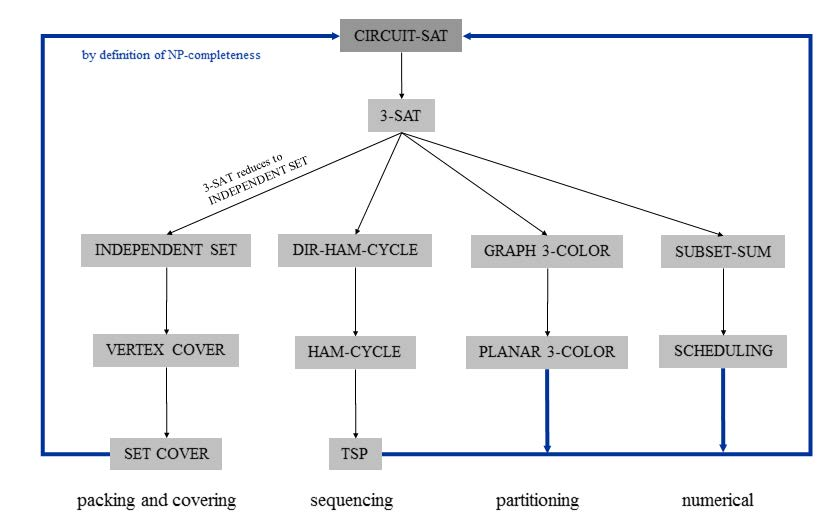
\includegraphics[width=\textwidth]{NPReduction.jpg}

\end{tcolorbox}

\end{multicols}
\end{document}
